\chapter{Realisation}

In the following chapter I talk about the development process of the system.

\section{Language, framework, toolkit}

There are many programming languages, frameworks and libraries that I considered when choosing my toolkit.

I wanted the server to be able to run on Linux because it is open source and free, so there is no need to buy a license for the operating system of choice. I expect our university to have Linux servers that they can use to run the server or a virtual machine can be created anywhere that runs Linux, without the need to run a UI.

I chose C++ and Qt as a platform. I decided not to use Microsoft technologies, .NET and C\# because even though they are opening to Linux, I believed C++ and Qt was a better, more supported option. I did not want to go with Java because C++ is much faster and more suited for algorithmically complex tasks. The solver could have used a declarative language like Prolog or Erlang, but I wanted to store the information in a database which is not very convenient in these languages. Qt is a suitable choice for the client since it supports multiple platforms seamlessly, so it can run on Windows and Linux as wanted.

I choose PostgreSQL as a database driver. I needed something that works seamlessly on Linux and can run separately from the server. This way the database can be installed on a computer with good network connections and large storage capabilities, independently of the server and the client. The database has to be online continuously so the client can upload new data to it while the server needs to be run only once.

Several libraries can be used for constraint programming. I chose Google's OR-tools because it is completely open source and it has multiple algorithms implemented in it, like linear programming plus many graph algorithms which makes it a versatile tool for operations research.

\section{Data model}

I assumed that the data model would be suspect to several changes as I develop the solver. In retrospect, this was true.

I wanted to create a framework where I could quickly change my data model depending on my needs and iterate over the different versions. I needed the data to be persistent and to have matching database tables and queries in SQL for manipulation.

To achieve this, I created a json format to describe my data.

The following format describes the C++ and SQL equivalent for every type in my system.

\begin{lstlisting}
{
    "id": {
        "cpp": "int", 
        "sql": "SERIAL PRIMARY KEY",
        "default_value": "0"
    },
    "reference": {
        "cpp": "int",
        "sql": "INTEGER",
        "default_value": "0"
    },
    "int": {
        "cpp": "int",
        "sql": "INTEGER",
        "default_value": "0"
    },
    "double": {
        "cpp": "double",
        "sql": "DOUBLE PRECISION",
        "default_value": "0.0"
    },
    "text": {
        "cpp": "std::string",
        "sql": "TEXT",
        "default_value": "\"\""
    },
    "bool": {
        "cpp": "bool",
        "sql": "BOOLEAN",
        "default_value": "false"
    },
    "timestamp": {
        "cpp": "std::string",
        "sql": "TIMESTAMP",
        "default_value": "\"\"" 
    }
}
\end{lstlisting}

Then, using these types the json file below describes my data model.

\begin{lstlisting}
{
    "default": {
        "members": [
            {
                "name": "modified_timestamp",
                "type": "timestamp"
            },
            {
                "name": "is_deleted",
                "type": "bool"
            }
        ]
    },
    "classes": [
        {
            "class": "timeslot",
            "members": [
                {
                    "name": "name",
                    "type": "text"
                }
            ],
            "references": []
        },
        {
            "class": "location",
            "members": [
                {
                    "name": "name",
                    "type": "text"
                }
            ],
            "references": []
        },
        {
            "class": "class_type",
            "members": [
                {
                    "name": "name",
                    "type": "text"
                }
            ],
            "references": []
        },
        {
            "class": "year",
            "members": [
                {
                    "name": "name",
                    "type": "text"
                }
            ],
            "references": []
        },
        {
            "class": "room",
            "members": [
                {
                    "name": "name",
                    "type": "text"
                },
                {
                    "name": "size_type",
                    "type": "text"
                }
            ],
            "references": [
                {
                    "class": "location"
                },
                {
                    "class": "class_type"
                }
            ]
        },
        {
            "class": "department",
            "members": [
                {
                    "name": "name",
                    "type": "text"
                },
                {
                    "name": "short_name",
                    "type": "text"
                }
            ],
            "references": []
        },
        {
            "class": "course",
            "members": [
                {
                    "name": "name",
                    "type": "text"
                }
            ],
            "references": [
                {
                    "class": "year"
                },
                {
                    "class": "department"
                }
            ]
        },
        {
            "class": "class",
            "members": [
                {
                    "name": "name",
                    "type": "text"
                }
            ],
            "references": [
                {
                    "class": "class_type"
                },
                {
                    "class": "course"
                }
            ]
        },
        {
            "class": "faculty_member",
            "members": [
                {
                    "name": "name",
                    "type": "text"
                }
            ],
            "references": [
                {
                    "class": "department"
                }
            ]
        },
        {
            "class": "license",
            "members": [],
            "references": [
                {
                    "class": "course"
                },
                {
                    "class": "class_type"
                },
                {
                    "class": "faculty_member"
                }
            ]
        }
    ]
}
\end{lstlisting}

Every class has an id member which is the primary key in the database table for that class. Then, the default section describes the members every class has, namely the last modification timestamp and a delete toggle for soft deletion.

The next section describes my classes. The timeslot is responsible for storing the different class periods (for example, Monday 8 am to 10 am, or Friday 10 am to 12 pm). The location class stores the buildings. The class type stores if the class is a seminar or practice session or a laboratory class. Year describes the different student years in the computer engineering major. Room stores the rooms on campus, which references the location the room is in and the type of class the room can hold. Department stores the faculty's departments. Course stores the different courses that are offered for the major (for example, Probability Theory or Theory of Algorithms). Class stores all the classes that are available from a specific course. The faculty member stores the teachers, referencing the department they are part of. The license indicates if a faculty member can teach a course, of the given class type.

\section{Automatic code generation}

Using these json descriptors, I wrote a Python script that generates the corresponding C++ classes and the database class responsible for interfacing to the PostgreSQL database. This way every time the data model changed throughout the development of the solver algorithm I was able to quickly change the json descriptor and generate a persistent data model for it without spending days changing the code manually.

Then I created a Google Drive Sheet for the data model, seen in Figure \ref{fig:GoogleDriveSheet}.

\begin{figure}[!ht]
\centering
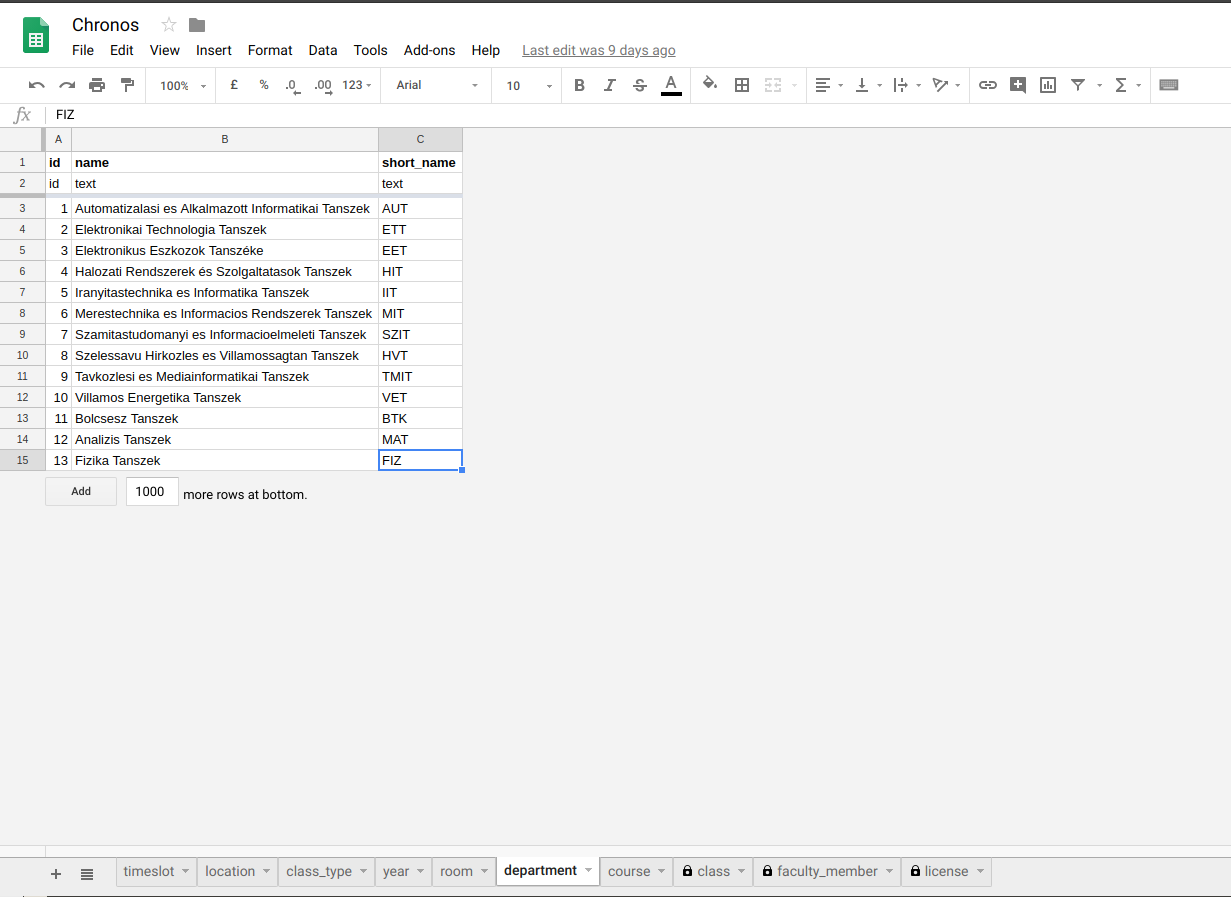
\includegraphics[width=\linewidth, keepaspectratio]{figures/chronos_sheet.png}
\caption{Google Drive Sheet} 
\label{fig:GoogleDriveSheet}
\end{figure}

The worksheets represent the classes in the data model. The first row lists the names of the variables, the second row the types of them. After that, every row is one object from the class or one row in the database. I wrote a Google Apps Script that will generate the descriptor jsons and an SQL script that creates the database structure and initialises the tables with the data from the worksheets.

Now, every time I needed to change the data model or the specific object I was able to open this spreadsheet, quickly edit it the way I wanted to, then run a few generator scripts and have my database ready and code modified to match it.

This quick prototyping method allowed me to make changes faster throughout the semester and played a huge role in completing my thesis on time.

\section{Mathematical description of the problem}

In the following section I will describe the Constraint Satisfaction Problem that I used to solve the timetabling problem.

Let $c_c$ denote the number of classes, $t_c$ the number of timeslots $r_c$ the number of rooms, $f_c$ the number of faculties and $p_c$ the number of allowed parallel non-seminar classes.\\

\subsection{Variables}

The variables are assigned in the following way.\\
\\
$T_i$ is the timeslot assigned to the ith class where $1\leq{}i\leq{}c_c$.\\
$R_i$ is the room assigned to the ith class where $1\leq{}i\leq{}c_c$.\\
$F_i$ is the faculty member assigned to the ith class where $1\leq{}i\leq{}c_c$.\\
\\
Then, there are special uniqueness variables. These variables help us to describe unique constraints in the system.  \\
\\
$U_{TR_i}$ is a uniqueness variable on the timeslot and room pair assigned to the ith class where $1\leq{}i\leq{}c_c$. These variables make sure rooms are not overbooked in any timeslot.\\\\
$U_{TF_i}$ is a uniqueness variable on the timeslot and faculty member pair assigned to the ith class where $1\leq{}i\leq{}c_c$. These variables make sure the faculty members don't have to teach two classes at the same time.\\\\
$U_{TYP_{i,j}}$ is a uniqueness variable on the timeslot, year and parallelness triplet assigned to the ith class where $1\leq{}i\leq{}c_c$ and jth parallel timeslot where $1\leq{}j\leq{}p_c$. These variables make sure that no year of students has to go to two classes at the same time.\\\\
$P_{i}$ is a parallelness variable for non-seminar classes. This allows the years of students to have parallel non-seminar classes in their timetable. \\

\subsection{Domains}

The domains of the variables are as follows.\\
\\
$T_i \in{} (1,t_c)$\\
$R_i \in{} (1,r_c) \cap \{$''where the room type matches the course type''$\}$\\
$F_i \in{} (1,f_c) \cap \{$''which class the faculty member is licensed to teach''$\}$\\
\\
$U_{TR_i} \in{} (1, (t_c + 1) (r_c + 1))$, $1\leq{}i\leq{}c_c$\\
$U_{TF_i} \in{} (1, (t_c + 1) (f_c + 1))$, $1\leq{}i\leq{}c_c$\\
$U_{TYP_{i,j}} \in{} (1, (t_c + 1) (y_c + 1) (p_c + 1))$, $1\leq{}i\leq{}c_c$, $1\leq{}j\leq{}c_c$\\

\subsection{Constraints}

The constraints are below.\\
\\
The uniqueness variables are number pairs represented as one number in a $t_c$ base-number system.\\
\\
$U_{TR_i} = R_i (t_c + 1) + T_i$\\
$U_{TF_i} = F_i (t_c + 1) + T_i$\\
\\
The $U_{TYP_i}$ variable uses the same representation trick but for a triplet.
When the ith class is a non-seminar class:\\
$U_{TYP_{i,1}} = Y_i (p_c + 1) (t_c + 1) + P_i (t_c + 1) + T_i$\\
\\
When the ith class is a seminar class we have to occupy ever parallel timeslot. This is done by creating $p_c$ number of uniqueness variables for seminars.\\
$U_{TYP_{i,j}} = Y_i (p_c + 1) (t_c + 1) + j (t_c + 1) + T_i$, $1\leq{}j\leq{}p_c$\\
\\
The following constraints make sure that the pairs and triplets are unique.\\
\\
AllDiff$(U_{TR_i})$ $\forall{}i$\\
AllDiff$(U_{TF_i})$ $\forall{}i$\\
AllDiff$(U_{TY_{i,j}})$ $\forall{}i,j$\\

\subsection{Optimalization}

To optimalize the devised timetable, I wanted to minimize the number of hole-hours for the students. To achieve this, we have to mathematically describe this using the variables in the Constraint Satisfaction Problem description above.

\paragraph{Theorem}

Let $S_1,S_2,...,S_{y_c}$ be the sets of the classes for a given year.

Minimizing $H_k = \sum\limits_{i\in{}S_k}\sum\limits_{j\in{}S_k}|T_i - T_j|$ will minimize the number of hole-hours in the kth year's timetable.

\paragraph{Lemma}

If the kth year's timetalbe with value $H_k = h$ contains a hole-hour there is always a timetable with value $H_k=h^*$ so that $h^* < h$.

\paragraph{Proof}

Let's move the chronologically first class, $min_{f}T_f$ in the timetable to the hole-hour. Then let's look at the changes in the $H_k$ value after this move. The $Y_i$, $Y_j$ pairs where $i\neq{}f$ and $j\neq{}f$ did not change, so their contribution to the sum did not change either.

The only pairs that changed are the ones where one of them was $T_f$.

Since $T_f$ was the first class, the value of $T_f$ could only increase when moved to the hole-hour.

Let $T_s$ denote the chronologically second class in the timetable. If we increase $T_f$'s value until $T_f = T_s$ the sum of every ($T_f$, $T_x$) pair's distances decreased, since $T_s\leq{}T_x$.

Then, let's denote the chornologically thrid class as $T_t$. If we increase  $T_f$'s value until $T_f = T_t$ there are two cases. The first case is with $T_s$. Since $T_f$ is getting further away from $T_s$, their distance is increasing. However, if we pair $T_s$ up with the chronologically last class, $T_l$, the sum of their distances from $T_f$ stays constant. The other case is with every other $T_x$, where the distance is decreasing.

We can continue this logic until a) we reach a hole-hour and put $T_f$ there, or b) until we leave the first half of the timetable.

In case a) we have successfully proven that the sum of all pairs's distances decreased by putting $T_f$ in the hole-hour. In case b) we know that hole-hour exists in the second half of the timetable. Here, we need to do the same process but instead of the chronologically first class we use the chronologically last and decrease its value, so from this viewpoint the hole-hour will be in the first half of the timetable.

This proves the correctness of the lemma.

Now, if for every timetable that contains a hole-hour we have proven that the $H_k$ value can't be minimal. This means that only timetables with no hole-hours can minimize the $H_k$ value, so minimizing for this results in hole-hour-less timetables.

This is the constraint I used for optimizing the timetables in the solver.

\section{Client}

The client is a simple Qt application, with minimal GUI.

The first picture shows the login screen of the application. I used PostgreSQL's user authentication. The database is installed on another computer, with IP 10.240.2.125.

\begin{figure}[!ht]
\centering
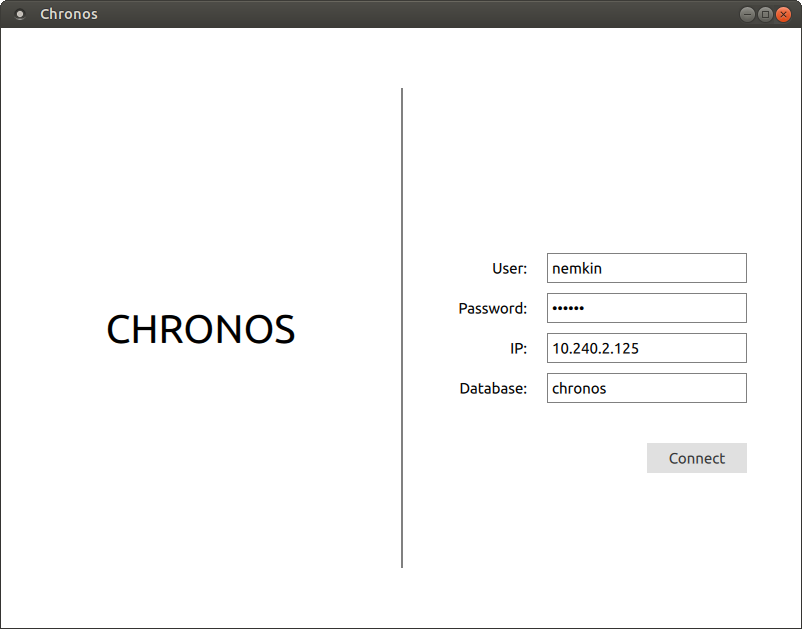
\includegraphics[width=\linewidth, keepaspectratio]{figures/login.png}
\caption{Login Screen} 
\end{figure}

The second picture shows the simple, basic GUI for the application, written in Qt.

\begin{figure}[!ht]
\centering
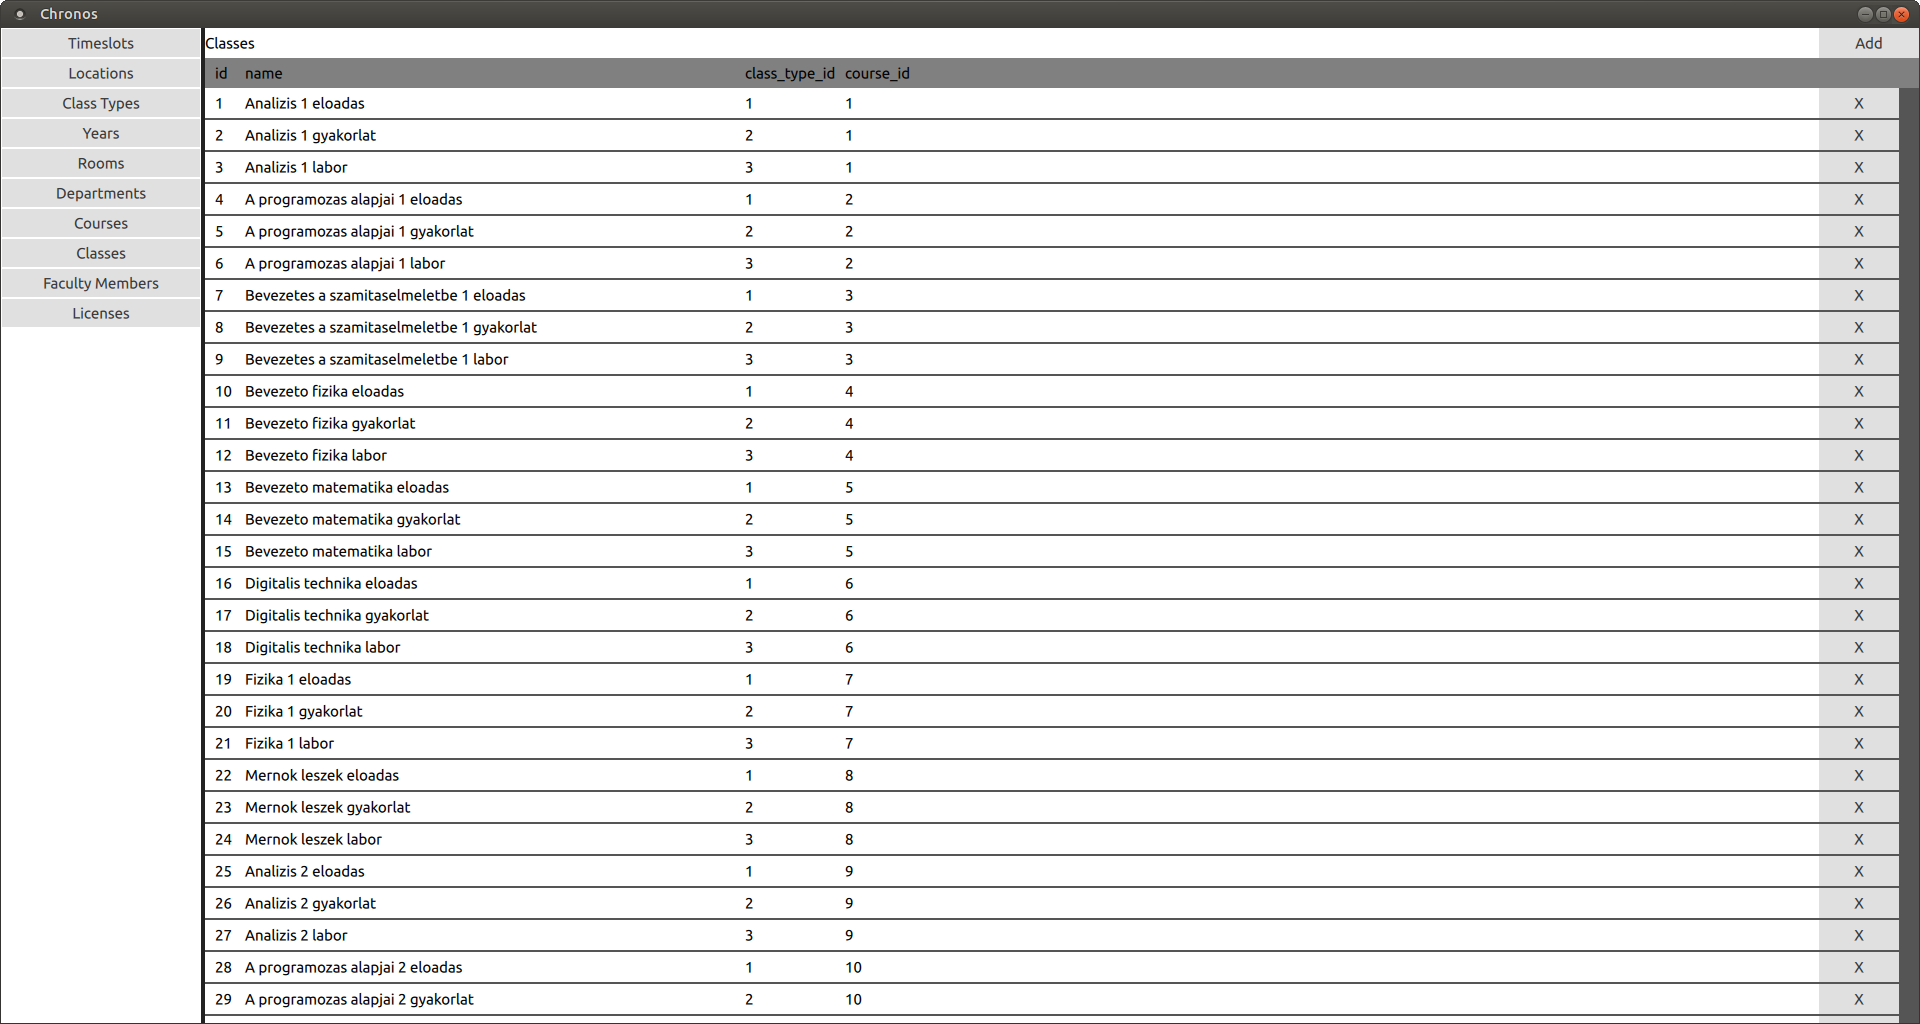
\includegraphics[width=\linewidth, keepaspectratio]{figures/inside.png}
\caption{Inside} 
\end{figure}

It can display the data, but currently it will not upload it back to the database.
